\begin{SCn}
	
\scnsectionheader{\currentname}
	
\scnstartsubstruct

\scntext{введение}{
В последнее десятилетие обозначилась устойчивая тенденция широкого применения методов машинного обучения в самых разных
областях человеческой деятельности, обусловленная в первую очередь развитием теории искусственных нейронных сетей(и.н.с.), а
также аппаратных возможностей.

Преимущество и.н.с. заключается в том, что они могут работать с неструктурированными данными.
Главный недостаток и.н.с. - это отсутствие понятной человеку обратной связи, которую можно было бы назвать цепочкой
рассуждений, т.е. можно сказать, что и.н.с. работают как ``черный ящик'' \scncite{gastelvecchi2016}.

Сложность современных интеллектуальных систем, использующих нейросетевые модели, а также большой объём обрабатываемых ими
данных обуславливают необходимость мониторинга, объяснения и понимания механизмов их работы с целью вербализации оценки
и оптимизации их деятельности.

В связи с этим становится актуальна разработка нейросимволических подходов(\scncite{nesy1}), в частности, подходов по интеграции и.н.с и баз знаний,
использующих онтологии. Такие интегрированные системы способны сочетать:

1) возможность семантической интерпретации обрабатываемых данных, используя представление решаемых и.н.с. прикладных задач,
а так же спецификацию её входных и выходных данных;

2) с представлением самой структуры и.н.с., описанием её свойств и состояний, позволяющими упростить понимание её работы(\scncite{ann_ostis2018}).

Можно выделить два основных направления интеграции и.н.с. с базами знаний:

1) построение интеллектуальных систем, способных использовать нейросетевые методы наравне с другими имеющимися в системе
методами для решения задач или подзадач системы. Такие системы смогут учитывать семантику решаемых задач на более высоком
уровне, что сделает решение этих задач более структурированными и прозрачными.

2) построение интеллектуальной среды по разработке, обучению и интеграции различных и.н.с., совместимых с базами знаний
через представление и.н.с. с помощью онтологических структур и их интерпретацию средствами представления знаний.
Такая среда предоставит возможност интроспекции и.н.с, возможность сохранения состояний и.н.с. после обучения и реконфигурации сети.
Это позволит производить более глубокий анализ работы и.н.с. Так же формальное описание знаний рамках предметной области
и.н.с. поможет поможет уменьшить порог вхождения разработчиков в методы решения задач с помощью и.н.с.

Данный раздел посвящен предметной области искусственных нейронных сетей, которая является основой развития обоих указанных направлений.
}

\scnheader{Предметная область искусственных нейронных сетей}
\scnidtf{Предметная область и.н.с.}
\scniselement{предметная область}
\scnsdmainclass{искусственная нейронная сеть;действие с искусственной нейронной сетью}
\scnsdclass{
    искусственная нейронная сеть;
    искусственная нейронная сеть с прямыми связями;
    персептрон;
    персептрон Розенблатта;
    персептрон Румельхарта;
    автоэнкодерная искусственная нейронная сеть;
    машина опорных векторов;
    искусственная нейронная сеть радиально-базисных функций;
    искусственная нейронная сеть с обратными связями;
    рекуррентная искусственная нейронная сеть;
    искусственная нейронная сеть Джордана;
    искусственная нейронная сеть Элмана;
    LSTM-элемент;
    GRU-элемент;
    полносвязная искусственная нейронная сеть;
    слабосвязная искусственная нейронная сеть;
    формальный нейрон;
    полносвязный формальный нейрон;
    сверточный формальный нейрон;
    рекуррентный формальный нейрон;
    синаптическая связь;
    параметр нейронной сети;
    настраиваемый параметр нейронной сети;
    весовой коэффициент;
    ядро свертки;
    архитектурный параметр нейронной сети;
    количество слоев;
    количество формальных нейронов;
    количество синаптических связей;
    паттерн входной активности н.с.;
    признак;
    слой и.н.с.;
    полносвязный слой и.н.с;
    сверточный слой и.н.с;
    слой и.н.с. нелинейного преобразования;
    dropout слой и.н.с.;
    pooling слой и.н.с.;
    действие обработки и.н.с.
}
\scnsdrelation{
    формальный нейрон\scnrolesign;
    пороговый формальный нейрон\scnrolesign;
    синаптическая связь\scnrolesign;
    входное значение формального нейрона*;
    выходное значение формального нейрона*;
    функция активации*;
    взвешенная сумма*;
    распределяющий слой*;
    обрабатывающий слой*;
    выходной слой*
}

\scnrelfrom{частная предметная область}{
Предметная область обучения искусственных нейронных сетей
}


%\scnrelfromset{частная предметная область}{
%Предметная область ИНС с заданным направлением связей\\
%    \scnaddlevel{1}
%    \scnrelfromset{частная предметная область}{
%    Предметная область ИНС с прямым связями\\
%        \scnaddlevel{1}
%        \scnrelfromset{частная предметная область}{
%        Предметная область персептронов\\
%            \scnaddlevel{1}
%            \scnrelfromset{частная предметная область}{
%            Предметная область персептронов Розенблатта
%            ;Предметная область персептронов Румельхарта
%            ;Предметная область автоэнкодерных ИНС
%            }
%            \scnaddlevel{-1}
%        ;Предметная область ИНС радиально-базисных функций
%        ;Предметная область машин опорных векторов
%        }
%        \scnaddlevel{-1}
%    ;Предметная область ИНС с обратными связями\\
%        \scnaddlevel{1}
%        \scnidtf{Предметная область рекуррентных ИНС}
%        \scnrelfromset{частная предметная область}{
%        Предметная область ИНС Джордана
%        ;Предметная область ИНС Элмана
%        ;Предметная область LSTM-элементов
%        ;Предметная область GRU-элементов
%        }
%        \scnaddlevel{-1}
%    }
%    \scnaddlevel{-1}
%;Предметная область обучения ИНС\\
%    \scnaddlevel{1}
%    \scnrelfromset{частная предметная область}{
%    Предметная область ИНС, обучающихся с учителем
%    ;Предметная область ИНС, обучающихся без учителя\\
%        \scnaddlevel{1}
%        \scnrelfromset{частная предметная область}{
%        Предметная область обучающихся автоэнкодерных ИНС
%        ;Предметная область ИНС глубокого доверия
%        ;Предметная область генеративно-состязательных ИНС
%        ;Предметная область самоорганизующихся карт Кохонена
%        ;Предметная область ИНС Хопфилда
%        ;Предметная область подкрепляющего обучения ИНС
%        }
%        \scnaddlevel{-1}
%    }
%    \scnaddlevel{-1}
%;Предметная область топологий ИНC\\
%    \scnaddlevel{1}
%    \scnrelfromset{частная предметная область}{
%    Предметная область полносвязных ИНC
%    ;Предметная область многослойных ИНC
%    ;Предметная область слабосвязных ИНC
%    }
%    \scnaddlevel{-1}
%;Предметная область задач, решаемых с помощью ИНС\\
%    \scnaddlevel{1}
%    \scnrelfromset{частная предметная область}{
%    Предметная область ИНС, решающих задачу классификации
%    ;Предметная область ИНС, решающих задачу аппроксимации
%    ;Предметная область ИНС, решающих задачу управления
%    ;Предметная область ИНС, решающих задачу фильтрации
%    ;Предметная область ИНС, решающих задачу детекции
%    ;Предметная область ИНС, решающих задачу с ассоциативной памятью
%    }
%    \scnaddlevel{-1}
%;Предметная область интеграции ИНС с базой знаний
%}

\scnheader{искусственная нейронная сеть}
    \scnidtf{и.н.с.}
    \scnidtf{множество искусственных нейронных сетей}
    \scnidtf{нейронная сеть}
    \scndefinition{
        \textbf{\textit{искусственная нейронная сеть}} -- это совокупность нейронных элементов и связей между ними (\scncite{Golovko2017}).

        Искусственная нейронная сеть состоит из \textbf{\textit{формальных нейронов}}, которые связаны между собой посредством
        \textbf{\textit{синаптических связей}}. Нейроны организованы в \textbf{\textit{слои}}. Каждый нейрон слоя принимает сигналы
        со входящих в него синаптических связей, обрабатывает их единым образом с помощью заданной ему или всему слою
        \textbf{\textit{функции активации}} и передает результат на выходящие из него синаптические связи.
    }
    \scnexplanation{
        \textbf{\textit{искусственная нейронная сеть}} -- это биологически инспирированная математическая модель,
        обладающая обобщающей способностью после выполнения процедуры обучения. Под обобщающей способностью понимается способность
        модели выдавать корректные результаты для паттернов входной активности, не входящих в обучающую выборку.
    }
    \scnsubset{математическая модель}
    \scnaddlevel{1}
        \scnexplanation{
            \textbf{\textit{математическая модель}} -- это упрощенное описание объекта реального мира, выраженное с
            помощью математической символики}
    \scnaddlevel{-1}

    \scnrelfrom{изображение}{
        \scnfileimage{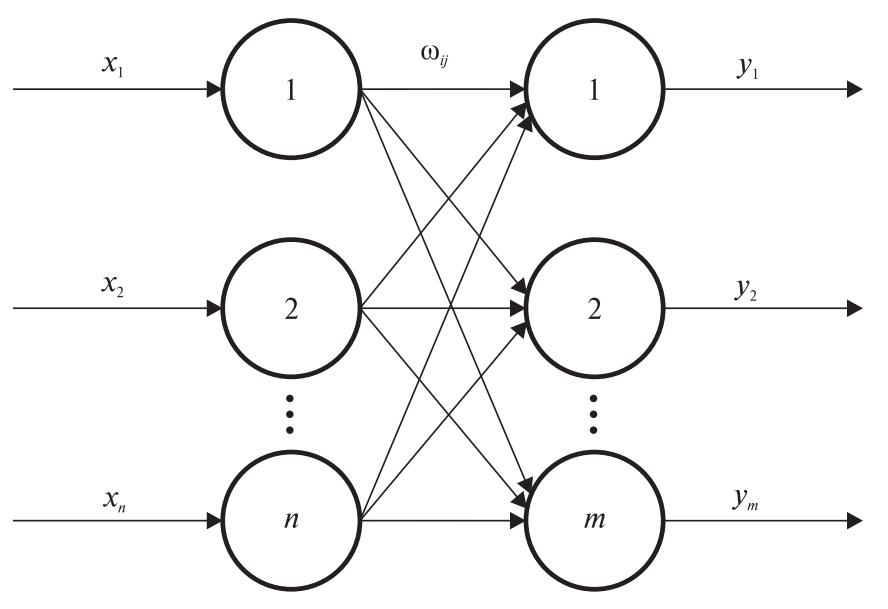
\includegraphics[width=0.4\linewidth]{figures/sd_ps/sd_ann/neural_network.png}}
    }

    \scnrelfrom{описание типичного экземпляра}{
        \scnfilescg{figures/sd_ps/sd_ann/neural_network_scg.png}
    }

    \scnrelfrom{разбиение}{\scnkeyword{Типология и.н.с. по признаку направленности связей\scnsupergroupsign}}
    \scnaddlevel{1}
        \scneqtoset{
        искусственная нейронная сеть с прямыми связями\\
        \scnaddlevel{1}
            \scnsubdividing{
                персептрон\\
                \scnaddlevel{1}
                    \scnsubdividing{
                        персептрон Розенблатта;
                        персептрон Румельхарта;
                        автоэнкодерная искусственная нейронная сеть
                    }
                \scnaddlevel{-1}
                ;машина опорных векторов
                ;искусственная нейронная сеть радиально-базисных функций
            }
        \scnaddlevel{-1}
        ;искусственная нейронная сеть с обратными связями
        \scnaddlevel{1}
            \scnidtf{рекуррентная искусственная нейронная сеть}
            \scnsubdividing{
            искусственная нейронная сеть Джордана
            ;искусственная нейронная сеть Элмана
            ;LSTM-элемент
            ;GRU-элемент
            }
        \scnaddlevel{-1}
        }
    \scnaddlevel{-1}

    \scnrelfrom{разбиение}{\scnkeyword{Типология и.н.с. по признаку полноты связей\scnsupergroupsign}}
    \scnaddlevel{1}
        \scneqtoset{
        полносвязная искусственная нейронная сеть\\
        ;слабосвязная искусственная нейронная сеть
        }
    \scnaddlevel{-1}

    \scnrelfrom{решаемые задачи}{задачи, которые могут быть решены с помощью и.н.с. с приемлемой точностью}{
    \scnaddlevel{1}
    \scneqtoset{
        задача классификации\\
        \scnaddlevel{1}
            \scnsubset{задача}
            \scnexplanation{задача построения классификатора, т.е. отображения $\tilde c: X \rightarrow C$, где $ X \in \mathbb{R}^m$ --
            признаковое пространство п.в.а., $C = {C_1, C_2, ...C_k }$ -- конечное и обычно небольшое множество меток классов.}
        \scnaddlevel{-1}
        ;задача регрессии\\
        \scnaddlevel{1}
            \scnsubset{задача}
            \scnexplanation{задача построения оценочной функции по примерам $(x_i, f(x_i))$, где $f(x)$ -- неизвестная функция}
            \scndefinition{\textbf{оценочная функция} -- отображение вида $\tilde{f}: X \rightarrow \mathbb{R}$, где $X \in \mathbb{R}^m$ -- признаковое пространство п.в.а.}
        \scnaddlevel{-1}
        ;задача кластеризация\\
        \scnaddlevel{1}
            \scnsubset{задача}
            \scnexplanation{задача разбиения множества п.в.а. на группы (кластеры) по какой-либо метрике сходства}
        \scnaddlevel{-1}
        ;задача понижения размерности\\
        \scnaddlevel{1}
            \scnsubset{задача}
            \scnidtf{задача уменьшения размерности признакового пространства}
        \scnaddlevel{-1}
        ;задача управления\\
        \scnaddlevel{1}
            \scnsubset{задача}
        \scnaddlevel{-1}
        ;задача фильтрации\\
        \scnaddlevel{1}
            \scnsubset{задача}
        \scnaddlevel{-1}
        ;задача детекции\\
        \scnaddlevel{1}
            \scnsubset{задача}
            \scnsubset{задача классификации}
            \scnsubset{задача регрессии}
        \scnaddlevel{-1}
        ;задача с ассоциативной памятью\\
        \scnaddlevel{1}
            \scnsubset{задача}
        \scnaddlevel{-1}
    }
    }

\scnheader{формальный нейрон}
    \scnidtf{искусственный нейрон}
    \scnidtf{нейрон}
    \scnidtf{ф.н.}
    \scnidtf{нейронный элемент}
    \scnidtf{множество нейронов искусственных нейронных сетей}
    \scnidtf{математическая модель реального биологического нейрона}
    \scnnote{отдельный формальный нейрон является искусственной нейронной сети с одним нейроном в единственном слое}
    \scnsubset{искусственная нейронная сеть}
    \scndefinition{
        \textbf{\textit{формальный нейрон}} -- это основной элемент \textit{искусственной нейронной сети}, применяющий свою \textit{функцию активации} к
            сумме произведений входных сигналов на весовые коэффициенты (\scncite{Golovko2017}):
        \begin{equation*}
            y = F\left(\sum_{i=1}^{n} w_ix_i\right) = F(WX)
        \end{equation*}
        где $X = (x_1,x_2,...,x_n)^{T}$ -- вектор входного сигнала; $W - (w_1,w_2,...,w_n)$ -- вектор весовых коэффициентов;
        \textit{F} -- функция активации.
    }

    \scnrelfrom{изображение}{
        \scnfileimage{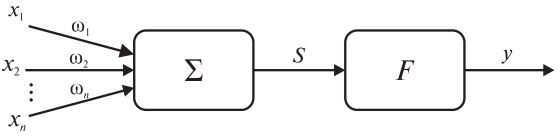
\includegraphics[width=0.4\linewidth]{figures/sd_ps/sd_ann/neuron.png}}
    }

    \scnnote{Формальные нейроны могут иметь полный набор связей с нейронами предшествующего слоя или неполный (разряженный)
        набор связей.}

    \scnsubdividing{
        полносвязный формальный нейрон\\
        \scnaddlevel{1}
            \scnidtf{нейрон, у которого есть полный набор связей с нейронами предшествующего слоя}
            \scnexplanation{отдельный обрабатывающий элемент и.н.с., выполняющий функциональное преобразование взвешенной суммы элементов вектора входных значений с помощью функции активации}
        \scnaddlevel{-1}
        ;сверточный формальный нейрон\\
        \scnaddlevel{1}
            \scnexplanation{отдельный обрабатывающий элемент и.н.с., выполняющий функциональное преобразование результата
                операции свертки матрицы входных значений с помощью функции активации}
            \scnnote{Сверточный формальный нейрон с соответствующим ему ядром свертки может быть представлен нейроном
                с неполным набором связей}
        \scnaddlevel{-1}
        ;рекуррентный формальный нейрон\\
        \scnaddlevel{1}
            \scnexplanation{формальный нейрон, имеющий обратную связь с самим собой или с другими нейронами и.н.с.}
        \scnaddlevel{-1}
    }

\scnheader{формальный нейрон\scnrolesign}
    \scnidtf{формальный нейронный элемент\scnrolesign}
    \scnidtf{нейронный элемент\scnrolesign}
    \scnidtf{нейрон\scnrolesign}
    \scniselement{ролевое отношение}
    \scnrelfrom{первый домен}{искусственная нейронная сеть}
    \scnrelfrom{второй домен}{формальный нейрон}
    \scnrelfrom{область определения}{искусственная нейронная сеть}
    \scndefinition{
        \textbf{\textit{формальный нейрон\scnrolesign}} -- ролевое отношение, связывающее искусственную нейронную сеть с ее нейроном.
    }

\scnheader{пороговый формальный нейрон\scnrolesign}
    \scnidtf{пороговый нейронный элемент\scnrolesign}
    \scnidtf{пороговый нейрон\scnrolesign}
    \scniselement{ролевое отношение}
    \scnrelfrom{первый домен}{искусственная нейронная сеть}
    \scnrelfrom{второй домен}{формальный нейрон}
    \scnrelfrom{область определения}{искусственная нейронная сеть}
    \scndefinition{
        \textbf{\textit{пороговый формальный нейрон\scnrolesign}} -- ролевое отношение, связывающее искусственную нейронную сеть с таким ее нейроном,
            выходное значение которого всегда равно -1.
    }
    \scnexplanation{весовой коэффициент синапса, выходящего из такого нейрона, является порогом для нейрона, в который
        данный синапс входит}

\scnheader{синаптическая связь}
    \scnidtf{синапс}
    \scnsubset{ориентированная пара}
    \scndefinition{
        \textbf{\textit{синаптическая связь}} -- ориентированная пара, первым компонентом которой является нейрон, из
        которого исходит сигнал, а вторым компонентом -- нейрон, который принимает этот сигнал.
    }

\scnheader{синаптическая связь\scnrolesign}
    \scnidtf{синапс\scnrolesign}
    \scniselement{ролевое отношение}
    \scnrelfrom{первый домен}{искусственная нейронная сеть}
    \scnrelfrom{второй домен}{синаптическая связь}
    \scnrelfrom{область определения}{
        ...\\
        \scnreltoset{объединение}{искусственная нейронная сеть;синапс}
    }
    \scndefinition{
        \textbf{\textit{синаптическая связь\scnrolesign}} -- ролевое отношение, связывающее искусственную нейронную сеть с ее синапсом.
    }

\scnheader{параметр и.н.с.}
    \scnsubset{параметр}
    \scnsubdividing{
        настраиваемый параметр и.н.с.\\
        \scnaddlevel{1}
            \scnidtf{параметр и.н.с., значение которого изменяется в ходе обучения}
            \scnsubdividing{
                весовой коэффициент синаптической связи;
                ядро свертки
                \scnaddlevel{1}
                    \scnidtf{квадратная матрица произвольного порядка, элементы которой изменяются в процессе
                        обучения и.н.с.}
                \scnaddlevel{-1}
            }
        \scnaddlevel{-1}\\
        ;архитектурный параметр и.н.с.\\
        \scnaddlevel{1}
            \scnnote{параметр и.н.с., определяющий ее архитектуру}
            \scnsubdividing{количество слоев;количество нейронов; количество синапсов}
        \scnaddlevel{-1}
    }

\scnheader{весовой коэффициент синаптической связи}
    \scnidtf{вес синапса}
    \scnidtf{сила синаптической связи}
    \scnsubset{настраиваемый параметр}
    \scnexplanation{
        \textbf{\textit{весовой коэффициент синаптической связи}} -- это числовой коэффициент, который ставится в соответствие каждому
        синапсу нейронной сети и изменяется в процессе обучения.
    }
    \scnnote{
        Если сила синаптической связи отрицательна, то она называется \textit{тормозящей}. В противном случае она
        является \textit{усиливающей}.
    }

\scnheader{входное значение формального нейрона*}
    \scnidtf{входное значение нейрона*}
    \scnidtf{входное значение*}
    \scniselement{неролевое отношение}
    \scniselement{бинарное отношение}
    \scnrelfrom{первый домен}{формальный нейрон}
    \scnrelfrom{второй домен}{число}
    \scnrelfrom{область определения}{
        ...\\
        \scnreltoset{объединение}{формальный нейрон;число}
    }
    \scndefinition{
        \textbf{\textit{входное значение формального нейрона*}} -- неролевое отношение, связывающее нейрон входного слоя со
        значением признака п.в.а., который подается на вход нейронной сети.
    }
    \scntext{теоретическая неточность}{
        Использование множества как формы представления входных данных является серьезным допущением, так как на практике
        входные данные структурированы более сложно -- в многомерные массивы. Самым близким теоретическим аналогом
        здесь выступает тензор. К сожалению, описание теории нейронных сетей с помощью тензорного исчисления в литературе
        как таковое отсутствует, но активно используется на практике: например, во многих разрабатываемых нейросетевых фреймворках.
        Формализация нейронных сетей с помощью тензоров видится авторам наиболее вероятным направлением работы в
        ближайших изданиях \textit{стандарта OSTIS}.
    }

\scnheader{паттерн входной активности и.н.с.}
	\scnidtf{п.в.а.}
    \scniselement{мультимножество}
    \scniselement{ориентированное множество}
    \scndefinition{
        \textbf{\textit{паттерн входной активности и.н.с.}} -- ориентированное мультимножество численных значений
        признаков некоторого объекта, которые могут выступать в качестве входных значений нейронов.
    }
	\scnnote{
        в текущей версии \textit{Стандарта OSTIS} предполагается, что п.в.а. содержит только предобработанные данные,
        то есть данные приведенные к численному виду и, возможно, преобразованные с помощью известных статистических
        методов (например, нормирования)
    }

\scnheader{признак}
    \scnidtf{feature}
    \scnidtf{множество признаков}
    \scnsubset{ролевое отношение}
    \scnexplanation{
        \textbf{\textit{признак}} -- множество ролевых отношений, каждое из которых связывает некоторый п.в.а. с численным значением, которое характеризует данный п.в.а. с какой-либо стороны.
    }

\scnheader{функция активации*}
    \scnidtf{функция активации нейрона*}
    \scniselement{неролевое отношение}
    \scniselement{бинарное отношение}
    \scndefinition{
        \textbf{\textit{функция активации*}} -- неролевое отношение, связывающее формальный нейрон с функцией, результат
        применения которой к \textbf{\textit{взвешенной сумме нейрона}} определяет его \textbf{\textit{выходное значение}}.
    }
    \scnrelfrom{область определения}{
        ...\\
        \scnreltoset{объединение}{формальный нейрон;функция}
    }
    \scnrelfrom{первый домен}{формальный нейрон}
    \scnrelfrom{второй домен}{функция}
    \scnaddlevel{1}
    \scnsubdividing{
        линейная\\
        \scnaddlevel{1}
            \scnrelfrom{формула}{
                \begin{equation*}
                    y = kS
                \end{equation*}
                где \textit{k} -- коэффициент наклона прямой, \textit{S} -- в.с.
            }
        \scnaddlevel{-1}
        ;пороговая\\
        \scnaddlevel{1}
            \scnrelfrom{формула}{
                \begin{equation*}
                    y = sign(S) =
                    \begin{cases}
                        1, S > 0,\\
                        0, S \leq 0
                    \end{cases}
                \end{equation*}
            }
        \scnaddlevel{-1}
        ;сигмоидная\\
        \scnaddlevel{1}
            \scnrelfrom{формула}{
                \begin{equation*}
                    y = \frac{1}{1+e^{-cS}}
                \end{equation*}
                где \textit{с} > 0 -- коэффициент, характеризующий ширину сигмоидной функции по оси абсцисс, \textit{S} -- в.с.
            }
        \scnaddlevel{-1}
        ;гиперболический тангенс\\
        \scnaddlevel{1}
            \scnrelfrom{формула}{
                \begin{equation*}
                    y = \frac{e^{cS}-e^{-cS}}{e^{cs}+e^{-cS}}
                \end{equation*}
                где \textit{с} > 0 -- коэффициент, характеризующий ширину сигмоидной функции по оси абсцисс, \textit{S} -- в.с.
            }
        \scnaddlevel{-1}
        ;softmax\\
        \scnaddlevel{1}
            \scnrelfrom{формула}{
                \begin{equation*}
                    y_j = softmax(S_j) = \frac{e^{S_j}}{\sum_{j} e^{S_j}}
                \end{equation*}
                где $S_j$ -- в.с. \textit{j}-го выходного нейрона
            }
        \scnaddlevel{-1}
        ;ReLU\\
        \scnaddlevel{1}
            \scnrelfrom{формула}{
                \begin{equation*}
                    y = F(S) =
                    \begin{cases}
                        S, S > 0,\\
                        kS, S \leq 0
                    \end{cases}
                \end{equation*}
                где \textit{k} = 0 или принимает небольшое значение, например, 0.01 или 0.001.
            }
        \scnaddlevel{-1}
    }
    \scnaddlevel{-1}

\scnheader{взвешенная сумма*}
    \scnidtf{взвешенная сумма входных значений*}
    \scnidtf{в.с.}
    \scniselement{неролевое отношение}
    \scniselement{бинарное отношение}
    \scndefinition{
        \textbf{\textit{взвешенная сумма*}} -- неролевое отношение, связывающее формальным нейрон с числом, являющимся суммой
        произведений входных сигналов на весовые коэффициенты входящих в нейрон синапсов.
    }
    \scnrelfrom{область определения}{
        ...\\
        \scnreltoset{объединение}{формальный нейрон;число}
    }
    \scnrelfrom{первый домен}{формальный нейрон}
    \scnrelfrom{второй домен}{число}
    \scnrelfrom{формула}{
        \begin{equation*}
            S = \sum_{i=1}^{n} w_ix_i
        \end{equation*}
        где \textit{n} -- размерность вектора входных значений, $w_i$ -- \textit{i}-тый элемент вектора весовых
        коэффициентов, $x_i$ -- \textit{i}-тый элемент вектора входных значений.
    }

\scnheader{выходное значение формального нейрона*}
    \scnidtf{выходное значение нейрона*}
    \scnidtf{выходное значение*}
    \scniselement{неролевое отношение}
    \scniselement{бинарное отношение}
    \scnrelfrom{первый домен}{формальный нейрон}
    \scnrelfrom{второй домен}{число}
        \scnrelfrom{область определения}{
        ...\\
        \scnreltoset{объединение}{формальный нейрон;число}
        }
    \scndefinition{
        \textbf{\textit{входное значение*}} -- неролевое отношение, связывающее нейрон с числом, являющимся результатом применения
        функции активации нейрона к его взвешенной сумме.
    }
    \scnnote{
        Выходное значение нейрона является одним из входных сигналов для всех нейронов, в которые ведут выходящие из данного нейрона синапсы.
    }

\scnheader{слой и.н.с.}
    \scnidtf{слой}
    \scnidtf{слой искусственной нейронной сети}
    \scnidtf{множество слоев искусственных нейронных сетей}
    \scnnote{отдельный слой является искусственной нейронной сетью с одним слоем}
    \scnsubset{искусственная нейронная сеть}
    \scnexplanation{
        \textbf{\textit{слой и.н.с}}  -- это множество нейронных элементов, на которые в каждый такт времени
        параллельно поступает информация от других нейронных элементов сети (\scncite{Golovko2017})
    }
    \scnexplanation{
        \textbf{\textit{слой и.н.с.}} -- это множество формальных нейронов, осуществляющих параллельную независимую обработку
        вектора или матрицы входных значений
    }
    \scnnote{функция активации слоя является функцией активации всех формальных нейронов этого слоя}
    \scnnote{конфигурация слоя задается типом, количеством формальных нейронов, функцией активации}
    \scnnote{описание последовательности слоев и.н.с. с конфигурацией каждого слоя задает архитектуру и.н.с.}

    \scnsubdividing{
        полносвязный слой и.н.с.\\
        \scnaddlevel{1}
            \scnidtf{слой, в котором каждый нейрон имеет связь с каждым нейроном предшествующего слоя}
            \scnidtf{слой, в котором каждый нейрон является полносвязным}
        \scnaddlevel{-1}
        ;сверточный слой и.н.с.\\
        \scnaddlevel{1}
            \scnidtf{слой, в котором каждый нейрон является сверточным}
        \scnaddlevel{-1}
        ;слой и.н.с. нелинейного преобразования\\
        \scnaddlevel{1}
            \scnidtf{слой, осуществляющий нелинейное преобразование входных данных}
            \scnexplanation{как правило, выделяются в отдельные слои только в программных реализациях. Фактически
                рассматриваются как финальный этап расчета выходной активности любого нейрона -- применение функции
                активации}
            \scnnote{не изменяет размерность входных данных}
        \scnaddlevel{-1}
        ;dropout слой и.н.с.\\
        \scnaddlevel{1}
            \scnidtf{слой, реализующий технику регуляризации dropout}
            \scnnote{данный тип слоя функционирует только во время обучения и.н.с.}
            \scnexplanation{поскольку полносвязные слои имеют большое количество настраиваемых параметров, они
                подвержены эффекту переобучения. Один из способов устранить такой негативный эффект -- выполнить
                частичный отсев результатов на выходе полносвязного слоя. На этапе обучения техника dropout позволяет
                отбросить выходную активность некоторых нейронов с определенной, заданной вероятностью. Выходная
                активность ``отброшенных'' нейронов полагается равной нулю.}
        \scnaddlevel{-1}
        ;pooling слой и.н.с.\\
        \scnaddlevel{1}
            \scnidtf{подвыборочный слой}
            \scnidtf{объединяющий слой}
            \scnidtf{слой, осуществляющий уменьшение размерности входных данных}
        \scnaddlevel{-1}
        ;слой и.н.с. батч-нормализации\\
    }

\scnheader{распределяющий слой*}
    \scnidtf{входной слой*}
    \scniselement{неролевое отношение}
    \scniselement{бинарное отношение}
    \scndefinition{
        \textbf{\textit{распределяющий слой*}} -- неролевое отношение, связывающее искусственную нейронную сеть с ее слоем,
        нейроны которого принимают входные значения всей нейронной сети.
    }
    \scnrelfrom{область определения}{искусственная нейронная сеть}
    \scnrelfrom{первый домен}{искусственная нейронная сеть}
    \scnrelfrom{второй домен}{слой и.н.с.}

\scnheader{обрабатывающий слой*}
    \scniselement{неролевое отношение}
    \scniselement{бинарное отношение}
    \scndefinition{
        \textbf{\textit{обрабатывающий слой*}} -- неролевое отношение, связывающее искусственную нейронную сеть с ее слоем,
        нейроны которого принимают на вход выходные значения нейронов предыдущего слоя.
    }
    \scnrelfrom{область определения}{искусственная нейронная сеть}
    \scnrelfrom{первый домен}{искусственная нейронная сеть}
    \scnrelfrom{второй домен}{слой и.н.с}

\scnheader{выходной слой*}
    \scniselement{неролевое отношение}
    \scniselement{бинарное отношение}
    \scndefinition{
        \textbf{\textit{выходной слой*}} -- неролевое отношение, связывающее искусственную нейронную сеть с ее слоем,
        выходные значения нейронов которого являются выходными значениями всей нейронной сети.
    }
    \scnrelfrom{область определения}{искусственная нейронная сеть}
    \scnrelfrom{первый домен}{искусственная нейронная сеть}
    \scnrelfrom{второй домен}{слой и.н.с}

\scnheader{действие обработки и.н.с.}
    \scnidtf{действие с искусственной нейронной сетью}
    \scnsubset{действие}
    \scnexplanation{
        В зависимости от того, является ли искусственная нейронная сеть знаком внешней по отношению к памяти системы сущности,
        элементы множества действие обработки и.н.с. являются либо элементами множества \textbf{\textit{действие, выполняемое кибернетической
        системой в своей внешней среде}}, либо элементом множества \textbf{\textit{действие, выполняемое кибернетической системой
        в собственной памяти.
    }}.
    }
    \scnsubdividing{
        действие конфигурации и.н.с.\\
        \scnaddlevel{1}
        \scnsubdividing{
            действие создания и.н.с.
            ;действие редактирования и.н.с.
            ;действие удаления и.н.с.
            ;действие конфигурации слоя и.н.с.\\
            \scnaddlevel{1}
                \scnsubdividing{
                    действие добавления слоя в и.н.с.
                    ;действие редактирования слоя и.н.с.
                    ;действие удаления слоя и.н.с.
                    ;действие установки функции активации нейронов слоя и.н.с.
                    ;действие конфигурации нейрона в слое и.н.с\\
                    \scnaddlevel{1}
                        \scnsubdividing{
                            действие добавления нейрона в слой и.н.с.
                            ;действие редактирования нейрона в слое и.н.с.
                            ;действие удаления нейрона из слоя и.н.с.
                            ;действие установки функции активации нейрона в слое и.н.с.
                        }
                    \scnaddlevel{-1}
                }
            \scnaddlevel{-1}
        }
        \scnaddlevel{-1}
        ;действие конфигурации весовых коэффициентов и.н.с.\\
        \scnaddlevel{1}
            \scnsuperset{действие обучения и.н.с.}
            \scnsuperset{действие начальной инициализации весов и.н.с.}
            \scnaddlevel{1}
                \scnsuperset{действие начальной инициализации весов нейронов слоя и.н.с.}
                \scnaddlevel{1}
                    \scnsuperset{действие начальной инициализации весов нейрона и.н.с.}
                \scnaddlevel{-1}
            \scnaddlevel{-1}
        \scnaddlevel{-1}
        ;действие интерпретации и.н.с.
    }
    \scnnote{
        Действия обработки и.н.с осуществляет соответствующий коллектив агентов.
    }
    \scnexplanation{
        Так как в результате действий обработки и.н.с объект этих действий, конкретная и.н.с, может существенно меняться
        (меняется конфигурация сети, ее весовые коэффициенты), то и.н.с представляется в базе знаний как темпоральное объединение
        всех ее версий. Каждая версия является и.н.с. и темпоральной сущностью. На множестве этих темпоральных сущностей задается
        темпоральная последовательность с указанием первой и последней версии. Для каждой версии описываются специфичные знания.
        Общие для всех версий знания описываются для и.н.с, являющейся темпоральным объединением всех версий.
    }
    \scnaddlevel{1}
        \scnrelfrom{пример}{
            \scnfilescg{figures/sd_ps/sd_ann/temporal_neural_network_scg.png}
        }
    \scnaddlevel{-1}

\scnstartsubstruct
\scnheader{Предметная область обучения искусственных нейронных сетей}
\scnidtf{Предметная область обучения и.н.с.}
\scniselement{предметная область}
\scnsdmainclass{искусственная нейронная сеть;действие обучения и.н.с.}
\scnsdclass{
    метод обучения и.н.с.;
    метод обучения с учителем;
    метод обратного распространения ошибки;
    метод обучения без учителя;
    метод оптимизации;
    функция потерь;
    параметр обучения;
    скорость обучения;
    моментный параметр;
    параметр регуляризации;
    размер группы обучения;
    количество эпох обучения;
    выборка
}
\scnsdrelation{
    обучающая выборка\scnrolesign;
    тестовая выборка\scnrolesign;
    валидационная выборка\scnrolesign;
    метод обучения\scnrolesign;
    метод оптимизации\scnrolesign;
    функция потерь\scnrolesign
}

\scnheader{действие обучения и.н.с.}
    \scnidtf{действие обучения искусственной нейронной сети}
    \scnsubset{действие конфигурации весовых коэффициентов и.н.с.}
    \scndefinition{
        \textbf{\textit{действие обучения и.н.с.}} -- действие, в ходе которого реализуется определенный метод обучения
        и.н.с. с заданными параметрами обучения и.н.с, методом оптимизации и функцией потерь.
    }
%    TODO format items
    \scnrelfromset{известные проблемы}{
        \scnfileitem{
        Переобучение -- проблема, возникающая при обучении и.н.с., заключающаяся в том,
        что сеть хорошо адаптируется к п.в.а. из обучающей выборки, при этом теряя способность к обобщению.
        Переобучение возникает из-за применения неоправданно сложной модели при обучении и.н.с. Это происходит,
        когда количество настраиваемых параметров и.н.с. намного больше размера обучающей выборки. Возможные
        варианты решения проблемы заключаются в упрощении модели, увеличении выборки, использовании регуляризации
        (параметр регуляризации, техника dropout и т.д.).
        Обнаружение переобученности сложнее, чем недообученности. Как правило, для этого применяется
        кросс-валидация на валидационной выборке, позволяющая оценить момент завершения процесса обучения.
        Идеальным вариантом является достижение баланса между переобученностью и недообученностью.
        };
        \scnfileitem{
        Недообучение -- проблема, возникающая при обучении и.н.с., заключающаяся в том,
        что сеть дает одинаково плохие результаты на обучающей и контрольной выборках.
        Чаще всего такого рода проблема возникает при недостаточном времени, затраченном на обучение модели.
        Однако это может быть вызвано и слишком простой архитектурой модели либо малым размером обучающей
        выборки. Соответственно решение, которое может быть принято ML-инженером, заключается в устранении
        этих недостатков: увеличение времени обучения, использование модели с большим числом настраиваемых
        параметров, увеличение размера обучающей выборки, а также уменьшение регуляризации и более тщательный
        отбор признаков для обучающих примеров.
        }
    }
    \scnrelfrom{типичная семантическая окрестность}{
        \scnfilescg{figures/sd_ps/sd_ann/ann_trainning.png}
    }

\scnheader{выборка}
    \scnsubset{множество}
	\scndefinition{
        \textbf{\textit{выборка}} -- множество п.в.а., используемых в процессе обучения, тестирования
        и архитектурной настройки и.н.с.
    }

\scnheader{обучающая выборка\scnrolesign}
    \scnidtf{training set\scnrolesign}
    \scniselement{ролевое отношение}
    \scnrelfrom{первый домен}{действие обучения и.н.с.}
    \scnrelfrom{второй домен}{выборка}
    \scnrelfrom{область определения}{
        ...\\
        \scnreltoset{объединение}{действие обучения и.н.с.;выборка}
    }
    \scndefinition{
        \textbf{\textit{обучающая выборка\scnrolesign}} -- ролевое отношение, связывающиее дествие обучения и.н.с. с выборкой,
        используемой для изменения настраиваемых параметров и.н.с. в процессе ее обучения.
    }

\scnheader{тестовая выборка\scnrolesign}
    \scnidtf{test set\scnrolesign}
    \scniselement{ролевое отношение}
    \scnrelfrom{первый домен}{действие обучения и.н.с.}
    \scnrelfrom{второй домен}{выборка}
    \scnrelfrom{область определения}{
        ...\\
        \scnreltoset{объединение}{действие обучения и.н.с.;выборка}
    }
    \scndefinition{
        \textbf{\textit{тестовая выборка\scnrolesign}} -- ролевое отношение, связывающиее дествие обучения и.н.с. с выборкой,
        используемой для проверки обобщающей способности обученной и.н.с.
    }
    \scnnote{элементы контрольной выборки не используются в процессе обучения}

\scnheader{валидационная выборка\scnrolesign}
    \scniselement{ролевое отношение}
    \scnrelfrom{первый домен}{действие обучения и.н.с.}
    \scnrelfrom{второй домен}{выборка}
    \scnrelfrom{область определения}{
        ...\\
        \scnreltoset{объединение}{действие обучения и.н.с.;выборка}
    }
    \scndefinition{
        \textbf{\textit{валидационная выборка\scnrolesign}} -- ролевое отношение, связывающиее дествие обучения и.н.с. с выборкой,
        используемой для определения (настройки) архитектурных параметров и.н.с. и параметров обучения.
    }
    \scnnote{элементы валидационной выборки не используются в процессе обучения (не входят в обучающую выборку)}


\scnheader{метод обучения и.н.с.}
    \scnsubset{метод}
	\scndefinition{
        \textbf{\textit{метод обучения}} -- метод итеративного поиска оптимальных значений настраиваемых параметров и.н.с.,
        минимизирующих некоторую заданную функцию потерь.
    }
	\scnnote{
        Стоит отметить, что хотя целью применения метода обучения является минимизация функции потерь, ``полезность''
        полученной после обучения модели можно оценить только по достигнутому уровню ее обобщающей способности.
    }
	\scnsuperset{метод обучения с учителем}
	\scnaddlevel{1}
		\scndefinition{
            \textbf{\textit{метод обучения с учителем}} -- метод обучения с использованием заданных целевых переменных.
        }
		\scnsuperset{метод обратного распространения ошибки}
		\scnaddlevel{1}
			\scnidtf{м.о.р.о.}
			\scntext{алгоритм}{
				\begin{algorithm}[H]
					\KwData{$X$ -- данные, $Et$ -- желаемый отклик (метки), $E_m$ -- желаемая ошибка (в соответствии с выбранной функцией потерь)}
					\KwResult{обученная нейронная сеть \textit{Net}}
					инициализация весов \textit{W} и порогов \textit{T};\\
					\Repeat{$E<E_m$}{
						\ForEach{$x \in X$ \And $e \in Et$}{
							фаза прямого распространения сигнала: вычисляются активации для всех слоев и.н.с.;\\
							фаза обратного распространения ошибки: вычисляются ошибки для последнего слоя и всех предшествующих слоев;\\
							изменение настраиваемых параметров и.н.с. в соответствии с вычисленными ошибками;\\
						}
						вычисление общей ошибки E на данной эпохе;
					}	
				\end{algorithm}
            }
			\scnnote{
                м.о.р.о. использует заданный метод оптимизации и заданную функцию потерь для реализации фазы
                обратного распространения ошибки и изменения настраиваемых параметров и.н.с. Одним из самых распространенных
                методов оптимизации является метод стохастического градиентного спуска. Приведенный м.о.р.о. используется
                для реализации последовательного варианта обучения.
            }
			\scnnote{
                Следует также отметить, что несмотря на то, что метод отнесен к методам обучения с учителем, в случае
                использования м.о.р.о. для обучения автокодировщиков в классических публикациях он рассматривается как
                метод обучения без учителя, поскольку в данном случае размеченные данные отсутствуют.
            }
		\scnaddlevel{-1}
	\scnaddlevel{-1}
	\scnsuperset{метод обучения без учителя}
	\scnaddlevel{1}
		\scndefinition{
            \textbf{\textit{метод обучения без учителя}} -- метод обучения без использования заданных целевых переменных
            (в режиме самоорганизации)
        }
		\scnexplanation{
            В ходе выполнения алгоритма метода обучения без учителя выявляются полезные структурные свойства
            набора. Неформально его понимают как метод для извлечения информации из распределения, выборка для которого
            не была вручную аннотирована человеком (\scncite{Goodfellow2017}).
        }
	\scnaddlevel{-1}

\scnheader{метод обучения\scnrolesign}
    \scniselement{ролевое отношение}
    \scnrelfrom{первый домен}{действие обучения и.н.с.}
    \scnrelfrom{второй домен}{метод обучения и.н.с.}
    \scnrelfrom{область определения}{
        ...\\
        \scnreltoset{объединение}{действие обучения и.н.с.;метод обучения и.н.с.}
    }
    \scndefinition{
        \textbf{\textit{метод обучения\scnrolesign}} -- ролевое отношение, связывающиее дествие обучения и.н.с. с методом обучения,
        использующимся для обучения и.н.с. в рамках этого действя.
    }

\scnheader{метод оптимизации}
    \scnsubset{метод}
	\scndefinition{
        \textbf{\textit{метод оптимизации}} -- метод для минимизации целевой функции потерь при обучении и.н.с.
    }
	\scnrelfromlist{включение}{
		SGD\\
		\scnaddlevel{1}
			\scnidtf{стохастический градиентный спуск}
			\scnidtf{с.г.с.}
			\scnidtf{stochastic gradient descent}
			\scnnote{в методе стохастического градиентного спуска корректировка настраиваемых параметров и.н.с. выполняется в направлении максимального уменьшения функции стоимости, т.е. в направлении, противоположном вектору градиента функции потерь (\scncite{Haykin2006})} 
		\scnaddlevel{-1}
		;Nesterov method\\
		\scnaddlevel{1}
			\scnidtf{метод Нестерова}
			\scnnote{обучение методом с.г.с. иногда происходит очень медленно. Импульсный метод позволяет ускорить обучение, особенно в условиях высокой кривизны, небольших, но устойчивых градиентов или зашумленных градиентов. В импульсном методе вычисляется экспоненциально затухающее скользящее среднее прошлых градиентов и продолжается движение в этом направлении. Метод Нестерова является вариантом импульсного алгоритма, в котором градиент вычисляется после применения текущей скорости (\scncite{Goodfellow2017})}
		\scnaddlevel{-1}
		;AdaGrad\\
		\scnaddlevel{1}
			\scnidtf{adaptive gradient}
			\scnnote{данный метод по отдельности адаптирует скорости обучения всех настраиваемых параметров и.н.с., умножая их на коэффициент, обратно пропорциональный квадратному корню из суммы всех прошлых значений квадрата градиента (\scncite{Duchi2011})}
		\scnaddlevel{-1}
		;RMSProp\\
		\scnaddlevel{1}
			\scnidtf{root mean square propagation}
			\scnnote{данный метод является модификацией AdaGrad, которая позволяет улучшить его поведение в невыпуклом случае путем изменения способа агрегирования градиента на экспоненциально взвешенное скользящее среднее. Использование экспоненциально взвешенного скользящего среднего гарантирует повышение скорости сходимости после обнаружения выпуклой впадины, как если бы внутри этой впадины алгоритм AdaGrad был инициализирован заново (\scncite{Goodfellow2017})} 
		\scnaddlevel{-1}	
		;Adam\\
		\scnaddlevel{1}
			\scnidtf{adaptive moments}
			\scnnote{данный метод можно рассматривать как комбинацию RMSProp и AdaGrad (\scncite{Kingma2014}). Помимо усредненного первого момента, данный метод использует усредненное значение вторых моментов градиентов}
		\scnaddlevel{-1}
	}
	\scnnote{
        Успешность применения методов оптимизации зависит главным образом от знакомства пользователя с соответствующим
        алгоритмом (\scncite{Goodfellow2017}).
    }

\scnheader{метод оптимизации\scnrolesign}
    \scniselement{ролевое отношение}
    \scnrelfrom{первый домен}{метод обучения и.н.с.}
    \scnrelfrom{второй домен}{метод оптимизации}
    \scnrelfrom{область определения}{
        ...\\
        \scnreltoset{объединение}{метод обучения и.н.с.;метод оптимизации}
    }
    \scndefinition{
        \textbf{\textit{метод оптимизации\scnrolesign}} -- ролевое отношение, связывающиее метод обучения и.н.с. с методом оптимизации,
        использующимся для обучения и.н.с. с помощью данного метода.
    }

\scnheader{функция потерь}
    \scnsubset{функция}
	\scndefinition{
        \textbf{\textit{функция потерь}} -- функция, используемая для вычисления ошибки, рассчитываемой как разница между фактическим
        эталонным значением и прогнозируемым значением, получаемым и.н.с.
    }
    \scnrelfromlist{включение}{
		MSE\\
		\scnaddlevel{1}
			\scnidtf{mean square error}
			\scnidtf{средняя квадратичная ошибка}
			\scnrelfrom{формула}{
				\begin{equation*}
					MSE = \frac{1}{m} \sum_{i=1}^m (y_i - e_i)^2
				\end{equation*}
				где $y_i$ -- прогноз модели, $e_i$ -- ожидаемый (эталонный) результат, \textit{m} -- размерность выходного вектора
			}
		\scnaddlevel{-1}
		;BCE\\
		\scnaddlevel{1}
			\scnidtf{binary cross entropy}
			\scnidtf{бинарная кросс-энтропия}
			\scnrelfrom{формула}{
				\begin{equation*}
					BCE = -(e \log(y) + (1 - e)\log(1 - y))
				\end{equation*}
				где $y$ -- прогноз модели, $e$ -- ожидаемый (эталонный) результат: \textit{0} или \textit{1}
			}
			\scnnote{для бинарной кросс-энтропии в выходном слое и.н.с. будет находиться один нейрон}
		\scnaddlevel{-1}
		;MCE\\
		\scnaddlevel{1}
			\scnidtf{multi-class cross entropy}
			\scnidtf{мультиклассовая кросс-энтропия}
			\scnrelfrom{формула}{
				\begin{equation*}
					MCE = - \sum_{i=1}^m e_{i} \log(y_{i})
				\end{equation*}
				где $y_{i}$ -- прогноз модели, $e_i$ -- ожидаемый (эталонный результат), \textit{m} -- размерность выходного вектора
			}
			\scnnote{для мультиклассовой кросс-энтропии количество нейронов в выходном слое и.н.с. совпадает с количеством классов}
		\scnaddlevel{-1}
	}
	\scnnote{
        Для решения задачи классификации рекомендуется использовать бинарную или мультиклассовую кросс-энтропийную функцию потерь,
        для решения задачи регрессии рекомендуется использовать среднюю квадратичную ошибку.
    }

\scnheader{функция потерь\scnrolesign}
    \scniselement{ролевое отношение}
    \scnrelfrom{первый домен}{метод обучения и.н.с.}
    \scnrelfrom{второй домен}{функция потерь}
    \scnrelfrom{область определения}{
        ...\\
        \scnreltoset{объединение}{метод обучения и.н.с.;функция потерь}
    }
    \scndefinition{
        \textbf{\textit{функция потерь\scnrolesign}} -- ролевое отношение, связывающиее метод обучения и.н.с. с функцией потерь,
        использующимся для обучения и.н.с. с помощью данного метода.
    }

\scnheader{параметр обучения}
   \scnidtf{группа наиболее общих параметров метода обучения и.н.с.}
   \scnrelfromvector{состав группы параметров обучения}{
       скорость обучения\\
          \scnaddlevel{1}
              \scndefinition{
                \textbf{\textit{скорость обучения}} -- параметр, определяющий скорость изменения параметров и.н.с.
                в процессе обучения.
              }
          \scnaddlevel{-1}
       ;моментный параметр\\
          \scnaddlevel{1}
                \scnidtf{момент}
                \scnidtf{momentum}
                \scndefinition{
                    \textbf{\textit{моментный параметр}} -- параметр, используемый в процессе обучения для устранения
                    проблемы ``застревания'' алгоритма обучения в локальных минимумах минимизируемой функции потерь.
                }
                \scnexplanation{
                    При обучении и.н.с. частой является ситуация остановки процесса в определенной точке локального
                    минимума без достижения желаемого уровня обобщающей способности и.н.с. Для устранения такого
                    нежелательного явления вводится дополнительный параметр (момент) позволяющий алгоритму обучения
                    ``перескочить'' через локальный минимум и продолжить процесс.
                }
         \scnaddlevel{-1}
       ;параметр регуляризации\\
         \scnaddlevel{1}
             \scndefinition{
                \textbf{\textit{параметр регуляризации}} -- параметр, применяемый для контроля уровня переобучения и.н.с.
             }
             \scndefinition{
                \textbf{\textit{регуляризация}} -- добавление дополнительных ограничений к правилам изменения настраиваемых
                параметров и.н.с. с целью предотвратить переобучение.
             }
         \scnaddlevel{-1}
       ;размер группы обучения\\
         \scnaddlevel{1}
             \scndefinition{
                \textbf{\textit{размер группы обучения}} -- размер группы п.в.а., которая используется для изменения параметров
                и.н.с. на каждом элементарном шаге обучения.
             }
         \scnaddlevel{-1}
       ;количество эпох обучения\\
       \scnaddlevel{1}
       		\scndefinition{
                \textbf{\textit{эпоха обучения}} -- одна итерация алгоритма обучения, в ходе которой все обучающие п.в.а.
                из обучающей выборки были однократно использованы.
            }
       \scnaddlevel{-1}
   }

\scnendstruct

\scnendsubstruct \scnendcurrentsectioncomment

\end{SCn}